\section{Создание мобильного приложения}

В рамках данной аттестационной работы было разработано кроссплатформенное мобильное приложение системы вероятностного моделирования с использованием фреймворка Apache Cordova. Данное приложение можно скомпилировать на множество платформ, поддерживаемых Apache Cordova, в частности это: Tizen, webOS, Android, iOS, Blackberry, Samsung Bada и Windows Phone. Тестировалось приложение на платформе Android 4.0.4 Ice Cream Sandwich.

\subsection{Настройка окружения}
Перед началом процесса разработки мобильного приложения необходимо настроить окружение, установить необходимые библиотеки и средства разработки. Для начала, необходимо убедиться, что NodeJS уже установлен и доступен для использования:
\begin{lstlisting}
 $ nodejs --version
 $ npm --version
\end{lstlisting}

Обе команды необходимо выполнить в командной строке и убедиться в том, что они успешно выполнились. В противном случае необходимо установить необходимые программы. Далее, установим необходимые библиотеки и их зависимости:
\begin{lstlisting}
 $ npm install -g cordova
\end{lstlisting}

Данная команда скачает из репозитория npm файл package.json для проекта cordova, создаст файлы, относящиеся к проекту, установит все зависимости, необходимые для корректной работы данного фреймворка, а также создаст ссылки на исполняемые файлы. Результат работы этой команды отображен на рисунке \ref{npm_cordova}. После завершения скрипта в нашей системе появится возможность использовать Cordova CLI из любого места за счет глобальной пролинковки (атрибут -g в команде установки).

\begin{figure}[ht]
\center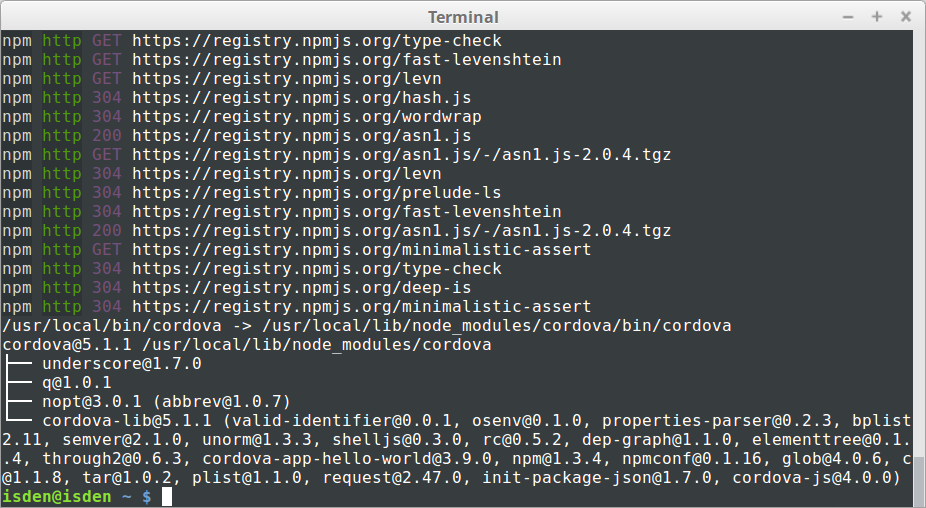
\includegraphics[width=0.9\textwidth]{npm_cordova}
\caption{Результат установки cordova}\label{npm_cordova}
\end{figure}

Для сборки проекта под Android необходимо установить и настроить Java SDK и Android SDK. Для этого скачиваем последние версии наборов разработки с официального сайта Oracle\cite{cordova:java_sdk} и официального сайта Google\cite{cordova:android_sdk}. Установка Java SDK не отличается ничем примечательным. После установки необходимо убедиться что правильно задана переменная окружения JAVA\_HOME.

Установка Android SDK отличается на различных платформах. Например, под ОС Windows необходимо запустить инсталлятор и следовать полученным инструкциям от мастера установки. Под ОС GNU\\Linux дистрибутив распространяется в качестве простого архива, который достаточно просто распаковать. После установки запускаем утилиту настройки \textit{android}, которая находится в каталоге platforms. Для сборки проекта в Apache Cordova необходимы Build Tools версии не ниже 19.0, а также ... не ниже ... . Пометим флажками для установки нужные компоненты (рисунок ), прочтем лицензионное соглашение и ожидаем окончания процесса скачивания и установки. После проведения данных манипуляций, необходимо убедиться в том, что в переменной PATH добавлен путь к каталогам ... и ... . Теперь все готово для начала процесса разработки.

\subsection{Адаптация приложения}
Для начала работ по переносу веб-приложения на мобильные устройства необходимо создать базовую структуру каталогов

\begin{figure}[ht]
\center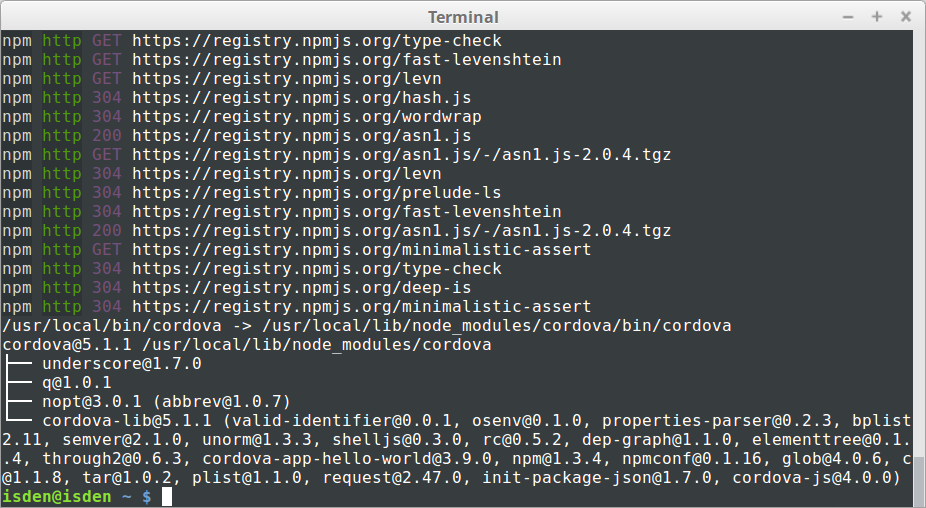
\includegraphics[width=0.9\textwidth]{npm_cordova}
\caption{Окно настройки средств разработки Android}\label{npm_cordova}
\end{figure}